\subsection{Sequence Diagram}

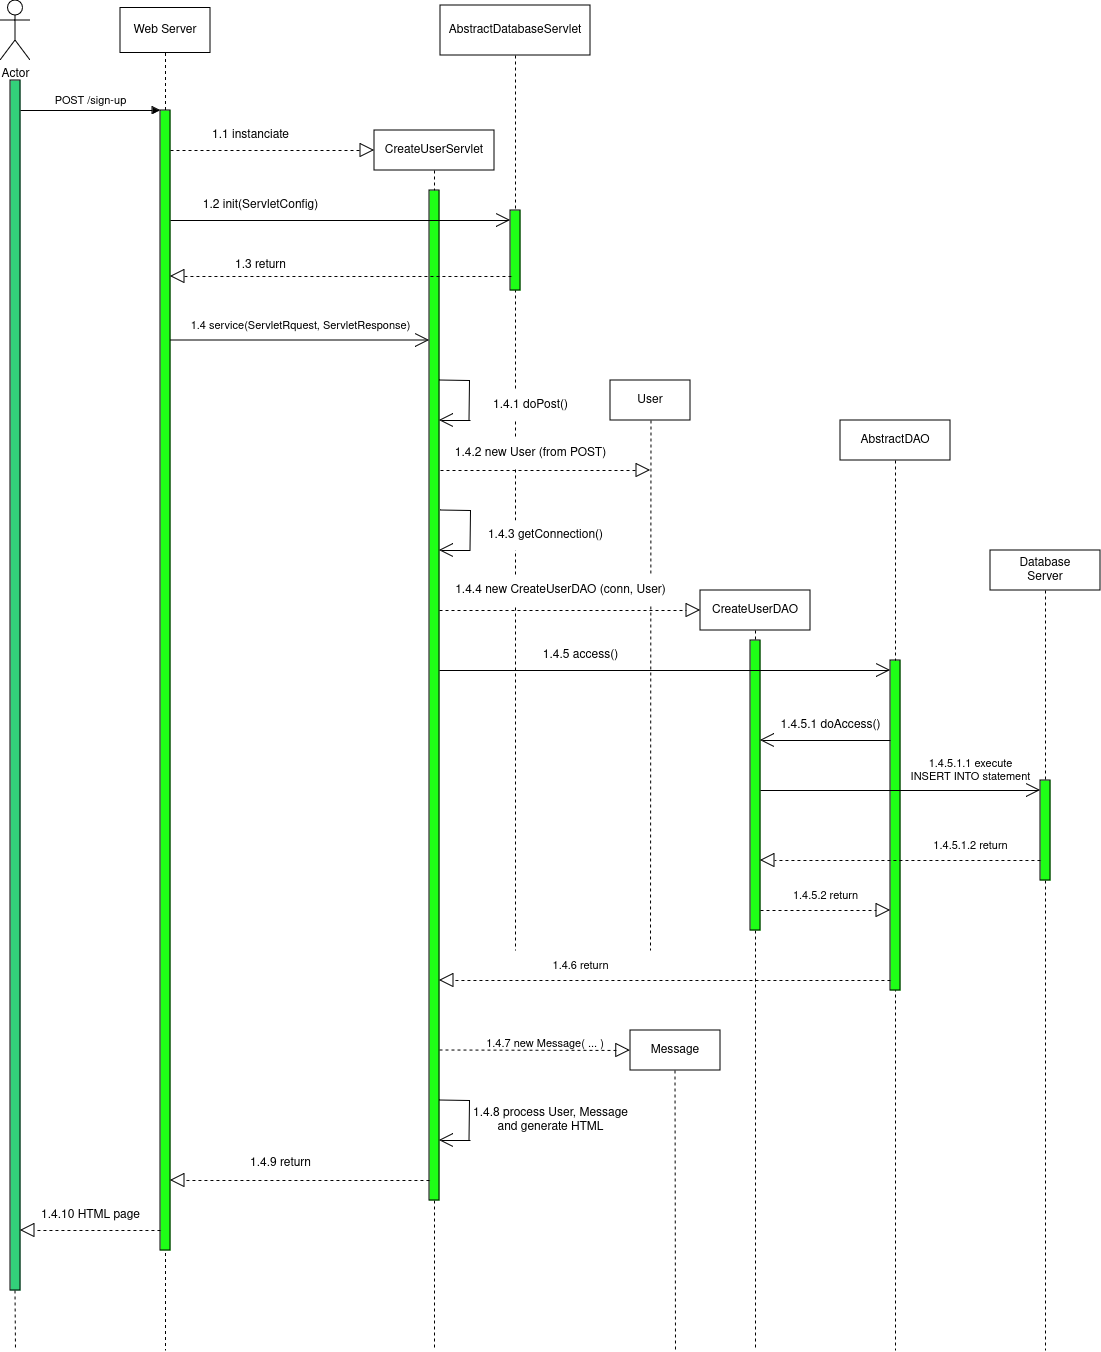
\includegraphics[width=0.85\linewidth]{seq_signup.png}
\newline
The sequence diagram explain what happens when a new user register on the website, operations which can be summarised in:
\begin{enumerate}
    \item The web server see a POST request on the link /sign-up and forward the request to the servlet mapped in that link, in this case CreateUserServlet.
    \item After initial configuration, the servlet creates a new User object with the data from the POST request received.
    \item This object is passed to the CreateUserDAO class, which execute the statement to insert that new user in the database.
    \item Once the DAO has done its job, the servlet check the reurn to see if everything went well and it creates a Message object to be displayed on the page and to be saved as log of that operation.
    \item The message is printed on a HTML page which is sent to the web server and then shown to the user.
\end{enumerate}
%describe here the sequence diagram